\documentclass[]{article}
\usepackage{url}
\usepackage{graphicx}
\usepackage{xcolor}
\usepackage[nodayofweek,level]{datetime}
\usepackage{textcomp}

\graphicspath{{./fig/}}
%opening
\title{OakNorth 2020 Machine Learning Initiatives}
\author{OakNorth Machine Learning}
\providecommand{\keywords}[1]{\textbf{\textit{Keywords---}} #1}
\providecommand{\values}[1]{\textbf{\textit{Value Proposition---}} #1}
\providecommand{\successmetric}[1]{\textbf{\textit{Success Metric---}} #1}
\newcommand{\toby}[1]{\textbf{\color{red}(Toby: #1)}}


\begin{document}

\maketitle
\begin{abstract}
    This document tracks down all initiatives that are driven by Machine 
    Learning and Statistics Modelling techniques in OakNorth. Each section 
    outlines an initiative, starting with a list of business stakeholders, 
    brief introduction of the task, dependencies of the initiative, and 
    potential client-facing applications that depend on it. Some will have 
    additional section to furthermore justify the initiative. The initiatives 
    in this document will be moved to ML JIRA board in a form of an 
    \textbf{EPIC} and 
    ready to be picked up by ML engineer(s) once it is approved by business 
    stakeholders.
    
    Each initiative is derived directly or indirectly from OakNorth 2020 
    vision\cite{oaknorth2020vision}. The ordering of the sections are     
    randomly chosen.
\end{abstract}
\section{Sentiments Analysis}

\keywords{Multi-class classification. Aspect based opinion mining.}

\subsection{Business Stakeholders}
Toby Smith

\subsection{Intro}
Being able to derive sentiments from text with respect to a borrower, 
product, or an industry, allows us to understand general opinion for the 
entity in question, from large stream of textual data efficiently. 
This alternative signal is shown to be an effective indicator for 
market movements \cite{bloomberg.com, bloomberg_quants}, or institution 
performance \cite{kasper2011sentiment, loughran2016textual}. Exposing 
sentiments derived from news, research and product reviews is beneficial 
for both our customer for monitoring purposes, and credit analysts for loan 
assessment. 


\subsection{Dependencies}
This initiative has dependencies on data, and optional dependencies on 
three other technical components. 

Different types of sentiments need slightly different types of data. 
Specifically:

\begin{enumerate}
    \item Subscription on Social Media feed, e.g. Twitter, Weibo (Company, 
    Sector and Sovereignty Sentiments)
    \item Subscription on News feed, e.g. Bloomberg EDF, Capital IQ Key 
    Development. (Sector and Sovereignty Sentiments)
    \item Subscription on Products reviews feed, e.g. Amazon/eBay/Yelp Products 
    Review. (Company, Sector and Sovereignty Sentiments)
\end{enumerate}

To derive company sentiments, we need \textbf{Named Entity 
Disambiguation}, s.t. we know what is the object for positive/negative 
sentiment in a paragraph. In this line of work, it is assumed that the corpus 
providing sentiment signals will have coverage on the companies. For news, 
however, it is rare SMEs are mentioned. Therefore the PI has to carefully 
decide what text corpus should we procure to derive SME sentiments.

To derive sector and sovereignty sentiments, we will 
need \textbf{Topic Classification}, so that we know what is the 
topic/sovereignty the text mainly concerns. Note that some vendors do 
provide topic classifications along with text so we may not need to build them 
in house. 

\subsection{Client Facing Applications}
\begin{enumerate}
    \item Sector Sentiments, Property Sentiments, etc.\textrightarrow 
    Monitoring
    \item Key Drivers Recommendation \textrightarrow Credit Analysis \& Tooling
\end{enumerate}


\newpage
\section{Table Understanding}

\keywords{Structured prediction. Information Extraction.}

\subsection{Business Stakeholders}
Kristjan Kaar,
Daria Saulenko

\subsection{Intro}
As stressed in vision document, extracting 
tables, understanding its structures and semantics, aka, converting data items 
to OakNorth taxonomy, are keys to automate 
borrower data extraction. Whilst works from ML team on Table Extraction and 
Structure Understanding have shown promising results that we can automate 
extracting and recovering tabular structures, our production system cannot 
automatically understand these tables, as 
\begin{enumerate}
    \item the data items in these files are named in higher degree of 
    variability
    \item calculation relationships in the sheets are not 
    captured.
    \item there are specific data items (e.g., Revenue from Solar Power 
    Storage in Tesla statement), and OakNorth taxonomy does not (and will 
    not\footnote{Company specific data items are less useful as it is hard to 
    use them for downstream tasks, such as benchmarking.}) have them.
\end{enumerate}

For example, in figure \ref{fig:tu_neighbour}, the current system can easily 
ingest \textbf{Revenues}, but not items such as \textbf{Contingent legal fees} 
as it is a 
specific item that OakNorth taxonomy does not contain. Nevertheless, for 
verification purpose, we still want to ingest the data item. We also want to 
automatically ingest the fact that data item \textbf{Contingent legal 
fees} contributes positively to calculation of \textbf{Total portfolio 
operations}, and negatively to calculation of \textbf{Net revenue (loss)}. 
These additional requirements cannot be handled by the current system.

In this initiative, we aim at zero-basing the table understanding model we have 
on production, and deliver a new system that can capture unknown data item and 
calculation dependencies across data items.  


\begin{figure}[h]
    \centering
    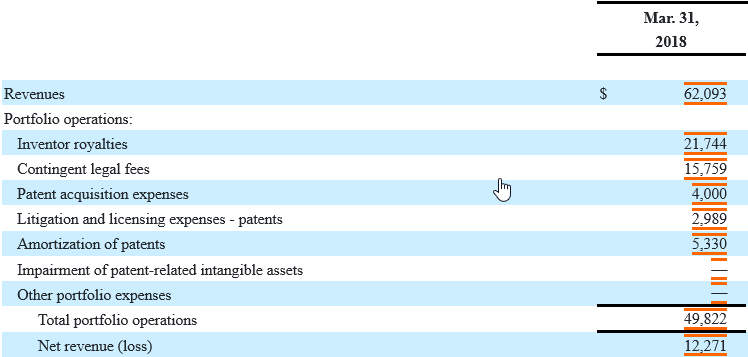
\includegraphics[width=.95\linewidth]{./tu_1.png}
    \caption{An extracted table from a SEC filing. The row starts with 
    \textbf{Contingent legal fees} are not recognised in OakNorth taxonomy, 
    while it contributes towards the calculation of \textbf{Total portfolio 
    operations} positively and \textbf{Net revenue (loss)}. 
    negatively. It is beneficial to ingest those data items as well for 
    verification purpose.\label{fig:tu_neighbour}}
\end{figure}

\subsection{Dependencies}
This initiative has dependencies on training data, the definition on OakNorth 
taxonomy, and dependencies among data items in OakNorth taxonomy. 

One recently available training corpus for this task is SEC iXBRL filings, 
which captures stylistic variations of tables in filings, representation 
differences on data items, and calculation dependencies among data items. An 
example can be 
seen in 
\url{https://www.sec.gov/ix?doc=/Archives/edgar/data/934549/000093454919000017/actg2018123110-k.htm}.

Note that, using SEC iXBRL filings as training data assumes that we can easily 
map OakNorth data items to US-GAAP data items. 

\subsection{Client Facing Applications}
\begin{enumerate}
    \item Raw Financials Ingestion \textrightarrow Internal Borrower Data 
    Ingestion
    \item  Raw Financials Ingestion \textrightarrow External Data Operation \& 
    Ingestion 
\end{enumerate}

\newpage

\section{Document Classification}
\keywords{Multi-class classification}
\subsection{Business Stakeholders}
Kristjan Kaar, Jagjit Sandhu
\subsection{Intro}
Relation managers for each borrower are required to classify each document 
uploaded by borrower to corresponding bucket, so that analysts can 
locate necessary information during credit assessment process faster. This 
manual categorisation process is time-consuming and repetitive. Given the fact 
that we already have large amount of bucketised documents in Nebula stack, can 
we build a system to automatically classify this document?

\subsection{Dependencies}
This initiative has one data and two technical dependencies. We require the 
bucketised raw borrower files from Nebula, which is used to be served by an 
SFTP, to be available on nebula production stack. For technical dependency, we 
need enclave \cite{ppdp2019on} to be ready, and document structure 
understanding to be ready. 

\subsection{Client Facing Applications}
\begin{enumerate}
    \item Document Upload \textrightarrow Credit Analysis \& Tooling
    \item Document Upload \textrightarrow Data Operation \& Ingestion
\end{enumerate}


\newpage

\section{Improvement on Peer Suggestion and Company Search}
\keywords{Learning to Rank, Time Series Modelling, NLP}
\\\\
\noindent
\values{As an RM, after borrower financials are ingested 
    and a sector selected, I am automatically presented a list of Peers for 
    comparison.}
\\\\
\noindent
\successmetric{Precision@K, Mean Average Precision, Normalised 
    Discounted Cumulative Gain.}
\subsection{Business Stakeholders}
Supratik Shankar, Jagjit Sandhu

\subsection{Intro}

The recently defined successful metric for peer suggestion system require a new 
set of manual annotations every time when a new baseline needs to be evaluated. 
At the moment, the collection of annotations are done in an-hoc excel 
workbooks. We crossed a point that we need a more systematic pipeline to 
improve and automate the process. 

On the other hand, with more annotations being collected, we can start 
investigating supervised modelling approach, e.g. Learning to Rank, to 
furthermore improve quality of suggested peers.

Finally, a closely related task, company search, can utilise the above 
annotation to improve the relevance of search results. 

This initiative tracks the effort of implementing an 
annotation pipeline, researching on (semi-)supervised approach on improving 
quality of peer suggestion, ranking of company search results, and 
productionisation of the outcome from the research.


\subsection{Client Facing Applications}
\begin{enumerate}
    \item Peer Suggestion \textrightarrow Credit Analysis \& Tooling, Monitoring
    \item Company Search \textrightarrow Credit Analysis \& Tooling, Monitoring
\end{enumerate}

\newpage

\section{Topic Classification}
\keywords{Multi-class classification, Structured prediction}
\\\\
\noindent
\values{For topics on borrower files: as an RM or Credit Analyst, I view an 
organized summary of key topics 
extracted from borrower documents; these are presented consistently 
post-ingestion within the borrower overview section.}
\\\\
\noindent
\successmetric{Macro F-score}

\subsection{Business Stakeholders}
Toby Smith, Morgan Williams

\subsection{Intro}
Classifying news, social media posts, and paragraphs in research reports or 
borrower submitted files to relevant topics are crucial for our clients to 
consume textual 
information in OakNorth platform. 
This allows them to quickly retrieve a piece of information they need, i.e. 
improve search engine, allow other algorithms such as sentiment analysis to 
correlate signals with
topics such as sovereignty, or business sectors. This initiative yields 

\begin{enumerate}
    \item A topic classification library that returns a set of topic codes 
    (with uncertainty)
    given parameters of domain and texts.
    \item A component in the ETL pipeline that enriches texts during ingestion.
    \item A new service in One-API that serves topic classification request.
\end{enumerate}
The library will associate each textual unit, defined by 
stakeholders\footnote{Textual unit has to be defined according to 
the kind of data. For example, it does not make 
sense to tag a full pdf file with 89 pages submitted from borrower w/ a set of 
topics as each page (or even a paragraph) can have very different topics. }, to 
a set of topic codes. The set of topic codes will differ from 
different kind of data\footnote{Topic codes have to be defined differently as 
some topic codes do not generalise to all kind of textual data. For 
example, a topic code such as "Fixed Charge" can be used to associate w/ a 
paragraph in borrower file which describes debt structure, while it is 
unintuitive to be used to tag a social media post}.

\subsection{Dependencies}
For topic classification on internal borrower files, the dependencies are

\begin{enumerate}
    \item Internal Borrower Files
    \item Definition of topics for borrower files
    \item Enclaves \cite{ppdp2019on}
    \item Document Structure Understanding
\end{enumerate}

For topic classification on external data, the dependencies are

\begin{enumerate}
    \item News/Social Media data on data platform.
    \item Definition of topics. e.g. Sovereignty and business sectors that we 
    are going to support.
\end{enumerate}

\subsection{Potential Topics}

From decision trees created by Analysts, we found out that flagging out the 
following paragraphs from a borrower file will be useful:

\begin{enumerate}
    \item Facility Amount
    \item Purpose of Loan
    \item Term
    \item Security (Collateral)
    \item Business Description
    \item Geography of Business
    \item Product Lists
    \item Utilisation details of past loans
    \item Management Information
    \item Legal Information
    \item Collaborator Details
    \item Group Structure
\end{enumerate}

\subsection{Client Facing Applications}
\begin{enumerate}
    \item News Search/Alerts \textrightarrow Monitoring
    \item Sentiments \textrightarrow Credit Analysis \& Tooling
    \item Data Operation \& Ingestion
\end{enumerate}

\newpage

\section{Content Search Engine}
\keywords{Learning to Rank, Information Retrieval}
\subsection{Business Stakeholders}
Jagjit Sandhu

\subsection{Intro}

Typical PDF viewer only allows users to search information by exact matching 
queries. As borrower submits tens of files, while each of them contains
hundreds of pages, it's hard and time-consuming for an analyst to retrieve 
relevant information. This effort tracks the implementation of a better ranker 
for search engine that, based on a query in logical form (or equivalents) 
\cite{may1985logical}, retrieve relevant textual units in multiple borrower 
files.

\subsection{Dependencies}
This effort depends on one data dependency, and four technology dependencies.

For data dependency, we need raw borrower files available on production stacks.

The technology dependencies are:

\begin{enumerate}
    \item Availability of Enclaves \cite{ppdp2019on}
    \item A search engine that indexes raw borrower files
    \item Named Entity Disambiguation
    \item Topic Classification
\end{enumerate}

\subsection{Client Facing Applications}
\begin{enumerate}
    \item Searching Raw Borrower Files \textrightarrow Credit Analysis \& 
    Tooling
    \item Searching Raw Borrower Files \textrightarrow Monitoring
\end{enumerate}

\newpage

\section{Named Entity Disambiguation}
\keywords{Structured prediction, Ranking}

\subsection{Business Stakeholders}
Morgan Williams

\subsection{Intro}
Named Entity Disambiguation (NED)\footnote{We use NED and Named Entity Linking 
interchangeably in this document} is a task of identifying what are the 
entities referred by sub-strings in a sentence, given a knowledge base (KB) of 
ground truth entities. Despite of the fact that NED is not directly 
client-facing, it is a crucial component for many down-stream applications, 
such as sentiments, content search engine, peers suggestion, etc. 

\subsection{Uniqueness}
Having a powerful NED can improve multiple components in OakNorth system 
vastly. For example, credit analysts can search mentions of a specific company 
(or all its subsidiary companies) across all submitted files from a borrower, 
even if the mentions are named with aliases or, worse, incompletely. NED with 
KB 
allows us to contextualise search\cite{voskarides2018weakly}\footnote{An 
illustrative example is: search Obama in Google and you will see relevant 
entities on the right side of the windows. } such that search results can be 
enriched. NED can be correlated with sentiment signals so that we can infer 
sentiment time-series for each company. 

Despite of the business values, to the authors' best knowledge, there is no 
commercial engine that can accurately link entities in text that mainly 
discusses about SME. 
One of the major reasons is lack of data to populate a SME centric KB to build 
NED, and, more importantly, NED is a notoriously 
difficult task \cite{hoffart-etal-2011-robust, ji2010overview, guo2014entity, 
globerson-etal-2016-collective}. Since OakNorth platform has access on text 
corpus from different SME business, and we have a strong in-house ML team for 
building proprietary NED algorithms, we will be in a good position to overcome 
the difficulties and obtain competitive advantages.

\subsection{Dependencies}
For data dependencies, the following types of data are required on KB

\begin{enumerate}
    \item Aliases Relationship
    \item Industry Relationship
    \item Company Descriptions Relationship
\end{enumerate}

The following are optional data dependencies on KB:

\begin{enumerate}
    \item Key Phrases/Tokens Relationship
    \item Company Website URL Relationship
    \item Supply Chain Relationship
    \item Co-occurrence Relationship
    \item Hyper Link Relationship
\end{enumerate}

Apart from the data dependencies from KB, the additional data dependencies are:

\begin{enumerate}
    \item Internal Borrower Files
    \item News/Social Media data on data platform.
\end{enumerate}

The technology dependencies are:

\begin{enumerate}
    \item A knowledge graph
    \item Document Structure Understanding
    \item Entity Consolidation
\end{enumerate}

\subsection{Client Facing Applications}
\begin{enumerate}
    \item Sentiments \textrightarrow Monitoring
    \item Content Search Engine \textrightarrow Credit Analysis \& Tooling
    \item News Search Engine \textrightarrow Monitoring
\end{enumerate}

\newpage


\section{News Search \& Recommendation Engine}
\keywords{Information Retrieval. Learning to Rank.}
\subsection{Business Stakeholders}
Toby Smith
\subsection{Intro}
While there will be millions of news flowing into the platform daily, we have 
to ensure that the information shown to clients is relevant, not 
redundant, and curtail to preferences of each individual. This 
initiative aims to build 
a search and recommendation system to allow clients to read the most relevant 
news with respect to their need, specified by query in logical form (or 
equivalents) \cite{may1985logical}.

\subsection{Uniqueness}
Overlaying real-time news with loans portfolio in a single dashboard is an 
extremely powerful feature, as this unified view helps users to quickly 
understand their portfolios from different sources in a single place, and 
a product like such with SME focus is the first of its kind in industry. 
Nevertheless, without a proper search engine to filter, refine, rank 
and recommend information, we will easily flood users with useless signals 
on the dashboard. This initiative is a core foundation to enable platform 
displaying news on dashboard. The algorithm yielded from this initiative will 
be an unique IP as it will be optimised specifically for SME.


\subsection{Dependencies}
For data dependencies, we would need News/Social media data available on data 
platform.

The following technology dependencies are mostly optional, in the sense that 
the lack of them does not block the completion of this initiative, while having 
them will lead to major improvements for search.

\begin{enumerate}
    \item Topic Classification
    \item Named Entity Disambiguation
    \item Sentiment Analysis
\end{enumerate}

\subsection{Client Facing Applications}
\begin{enumerate}
    \item Monitoring
\end{enumerate}

\newpage

\section{Key Drivers Recommendation}
\keywords{Quantitative Finance. Risk Factor Analysis.}
\\\\
\noindent
\values{The ON Platform provides explanations of returns 
(or other target financials) by fundamental drivers such as Macro Economic, 
Industry  KPIs. The estimated exposures w.r.t factors can then be used to 
formulate warnings (so that when the company is highly exposed to KPI x, and 
when there are warnings to X, a warning will be triggered for the borrower)}
\\\\
\noindent
\successmetric{ Performance of Backtesting for evaluating warning 
triggering.}

\subsection{Business Stakeholders}
Christopher Woon
\subsection{Intro}

In the process of credit analysis for SME lending, analysts are required to 
come up with a projection of the company performance to correctly evaluate the 
risk of such loan. This step, aka Financial Modelling, usually consists of 
three necessary stages

\begin{enumerate}
    \item Industry Review - Analysts read through news, past research, company 
    filings etc to understand the industry of the borrower.
    \item Analysts, based on experience and the outcome from industry review, 
    hand-pick several factors and hand-setting weights for the factors. 
    \item Review the fit
\end{enumerate}

Key-driver selection step is time-consuming, as this is very much experience 
driven and the learning curve of individual analyst is steep. Furthermore, the 
current selection step involves with a manual data collection and mental 
exercise to summarise key factors from quantitative and qualitative data. 

This initiative tries to build a model that can \textit{\textbf{suggest}} the 
most related key drivers with respect to a target variable of a base borrower, 
based on historical spreads, previously selected key-drivers by senior 
analysts, jointly with peer financials. The target variable can be proxy 
metrics of company performance, or it can be covenant. 

\subsection{Dependencies}
Here lists the data dependencies:
\begin{enumerate}
    \item Industry Data Time Series on Data Platform
    \item Company Financials
\end{enumerate}

Note that, as we want to have more explaining power, the frequency of 
time-series should be as high as possible, e.g. daily is better than quarterly.

The following are optional technology dependencies, as they can provide 
potential factors to be correlated w/ target financials by the recommendation 
algorithm:
\begin{enumerate}
    \item Sentiments \& Named Entity Disambiguation
    \item Sentiments \& Topic Classification
\end{enumerate}

Peer suggestion is another optional technology dependency, as it can provide a 
smaller estimation universe by suggesting a list of companies that is closest 
in terms of financial behaviours.

\subsection{Client Facing Applications}
\begin{enumerate}
    \item Alerting on Abnormality on Key Drivers \textrightarrow Monitoring
    \item Financial Modelling \textrightarrow Credit Analysis \& Tooling
    \item Suggesting news that relates to key drivers \textrightarrow Monitoring
\end{enumerate}

\newpage

\section{Entity Consolidation}
\keywords{Data alignment, Deduplication, Combinatorial Optimisation}
\\\\
\noindent
\values{Clients using our platform will not see duplicated companies from 
different data vendors we have. They will only see one that is consolidated.}
\\\\
\noindent
\successmetric{Precision \& Recall}
\subsection{Business Stakeholders}
Morgan Williams, Tiziano Quarantotto 

\subsection{Intro}
As we source data from multiple vendors, there will be duplicated information 
flowing into OakNorth. Since OakNorth data platform is entity centric, we have 
to consolidate information which refers to the same entity to avoid unwanted 
side-effects in downstream applications. This initiative aims to construct a 
generalised framework that can deduplicate among entities of the same type 
ingested from different vendors with probabilistic model(s). To start with, we 
will focus on consolidating information of companies sourced from Factset, 
Orbis, and Capital IQ. We will then extend the framework to deal with 
consolidating transactions and listings of properties.

\subsection{Dependencies}
The data dependencies are:

\begin{enumerate}
    \item Company data from at least two vendors.
    \item Historical property listing and transaction data.
\end{enumerate}

\subsection{Client Facing Applications}
All client facing applications, e.g. Credit Tooling, Monitoring, that retrieve 
entities from OneDB will be benefited vastly from this initiative.

\newpage


\section{Document Structure Understanding}
\keywords{Structured Prediction, Deep Learning, Computer Vision, Language 
Modelling}
\\\\
\noindent
\values{As a Data Analyst (at ON or a client), I have increased efficiency of 
ingesting financial data.}
\\\\
\noindent
\successmetric{Time to ingest a document}
\subsection{Business Stakeholders}
Kristjan Kaar, Ezgi Bereketli 
\subsection{Intro}
One of the major time blockers for credit analysts have been manual entries of 
data from raw files submitted from borrowers. This efforts aims at 
semi-automate the manual ingestion process by computer vision and language 
modelling techniques to 

\begin{enumerate}
    \item Segment the documents into different types of contents: Tables, 
    Paragraphs, Figures, etc.
    \item Understand the tabular structure of each table, i.e. segment the 
    table into MxN 
    cells according to visual evidence. This include retrieval of formatting 
    information. The system should also return how (un)certain the system is.
    \item OCR (Optic Character Recognition) to obtain the contents of the 
    tables from the pixels. OCR to obtain the texts of paragraphs.
    \item Detect the topics and saliency of the tables.
\end{enumerate} 

\subsection{Dependencies}

The optional dependencies are:
\begin{enumerate}
    \item Raw borrower files
    \item Enclaves \cite{ppdp2019on}
\end{enumerate}

\subsection{Client Facing Applications}
\begin{enumerate}
    \item Data Operation for Financials Extraction \textrightarrow Monitoring, 
    Credit Analysis \& Tooling
    \item Content Search Engine \textrightarrow Monitoring, Credit Analysis \& 
    Tooling
\end{enumerate}

\newpage


\section{Industry Classification}
\keywords{Structured Prediction, Deep Learning, Natural Language Processing, 
Multi-class classification}
\\\\
\noindent
\values{1. Clients using our platform can quickly pick sectors by entering 
keywords.  2. Most companies in DP does not have L6 OneClass classification 
code. We can improve coverage by prepopulating L6 code for all companies w/ 
description in the platform. This improves data consistency in our platform.}
\\\\
\noindent
\successmetric{Macro F-score}

\subsection{Intro}
Industry classification of a company is crucial analytics for OakNorth platform 
user to refine company and peer search results. As some companies are not 
tagged with their industries, this often leads to inferior search results. This 
initiative tracks the effort of implementing a Machine Learning classifier that 
infers industries code given company descriptions. Specifically, it yields

\begin{enumerate}
    \item A library that infer industries (with uncertainty) given company 
    descriptions.
    \item A new component in ETL pipeline that automatically tags companies 
    with their industry code.
    \item A new service in One-API that serves industry classification requests.
\end{enumerate}

\subsection{Dependencies}
This effort depends on the availiability of company dataset from Factset.
\subsection{Client Facing Applications}
\begin{enumerate}
    \item Automatically suggest industry code in credit bench when 
    borrower is filling in a new application.
    \item Peer Suggestion \textrightarrow Credit Analysis \& Tooling,  
    Monitoring
    \item Company Search \textrightarrow Credit Analysis \& Tooling,  Monitoring
\end{enumerate}
\newpage
\section{Information Extraction from Property Listings}
\keywords{Computer Vision, Deep Learning}
\subsection{Intro}
To evaluate a property loan, credit analysts needs to conduct a thorough 
analysis on the \textit{similar} properties of the area to verify the 
hypothesis suggested by the borrower. To measure similarity across different 
properties we have to extract information from unstructured listing data to aid 
the analysis, as they are not provided in standard feeds of property data 
vendors, while the premium feed is extremely expensive \footnote{Reach out to 
business stakeholders for the estimation of cost.}. The initiative tracks the 
effort of extracting crucial attributes of a property from unstructured data 
such as the webpage, floor plans or other attachments  of the listing. Here 
lists the set of attributes analysts are interested in:

\begin{enumerate}
    \item Square Footage
    \item Surrounding amenities
    \item No. of bedrooms, living rooms, gardens, parking, garage, lift, gated 
    community, concierge services, retirement property.
    \item whether the property is New Build, Old Build, Refurbished)
    \item Property Type (Detached, Semi-detached, Terrace, End of Terrace, 
    Bungalow)
    \item Sub-classification (1st/2nd Floor, lower ground floor, mezzanine 
    floor, penthouse)
    
\end{enumerate}

\subsection{Dependencies}

This initiative depends on the availability of historical property data. There 
is no known technology dependency.

\subsection{Client Facing Applications}
\begin{enumerate}
    \item Property Heat Map \textrightarrow Monitoring, Credit Analysis \& 
    Tooling
\end{enumerate}

\newpage



\bibliographystyle{unsrt}
\bibliography{main.bib}

\end{document}
